\chapter{面向微调鲁棒性的可持久性安全编辑机制}\label{chap:method}

\section{相关知识介绍}
本节为示例占位内容，用于演示公式、定理与插图的排版。请替换为实际内容。

公式应另起一行居中，编号按章编排并置于行末，如式~\eqref{eq:demo1} 与式~\eqref{eq:demo2}
所示：
\begin{equation}\label{eq:demo1}
  y = \sum_{i=1}^{n} a_i x_i + b.
\end{equation}
\begin{equation}\label{eq:demo2}
  f(x) = \int_{0}^{\infty} e^{-x t}\,\mathrm{d}t = \frac{1}{x}, \quad x>0.
\end{equation}

\begin{definition}[示例定义]\label{def:demo}
此处为示例定义的占位内容，用于演示定义环境的排版。
\end{definition}

\begin{theorem}\label{thm:demo}
此处为示例定理的占位内容，用于演示定理环境的排版。
\end{theorem}
\begin{proof}
此处为示例证明的占位内容，用于演示证明环境的排版。证毕。
\end{proof}

\subsection{参数级知识编辑范式}
% TODO: ROME / MEMIT / AlphaEdit 的定位-编辑机制回顾，参数编辑范式的特点。

\subsection{问题定义}
% TODO: 编辑对象、遗忘目标与约束条件的形式化定义。

\subsection{威胁模型}
% TODO: 良性微调与恶意微调双威胁设定；保持率 Retention(t)、攻击回潮率、护栏完整度的问题定义。

\section{方案框架}
本文方法的总体框架如图~\ref{fig:framework} 所示。图序号和图标题居中置于图下方。

\begin{figure}[htbp]
  \centering
  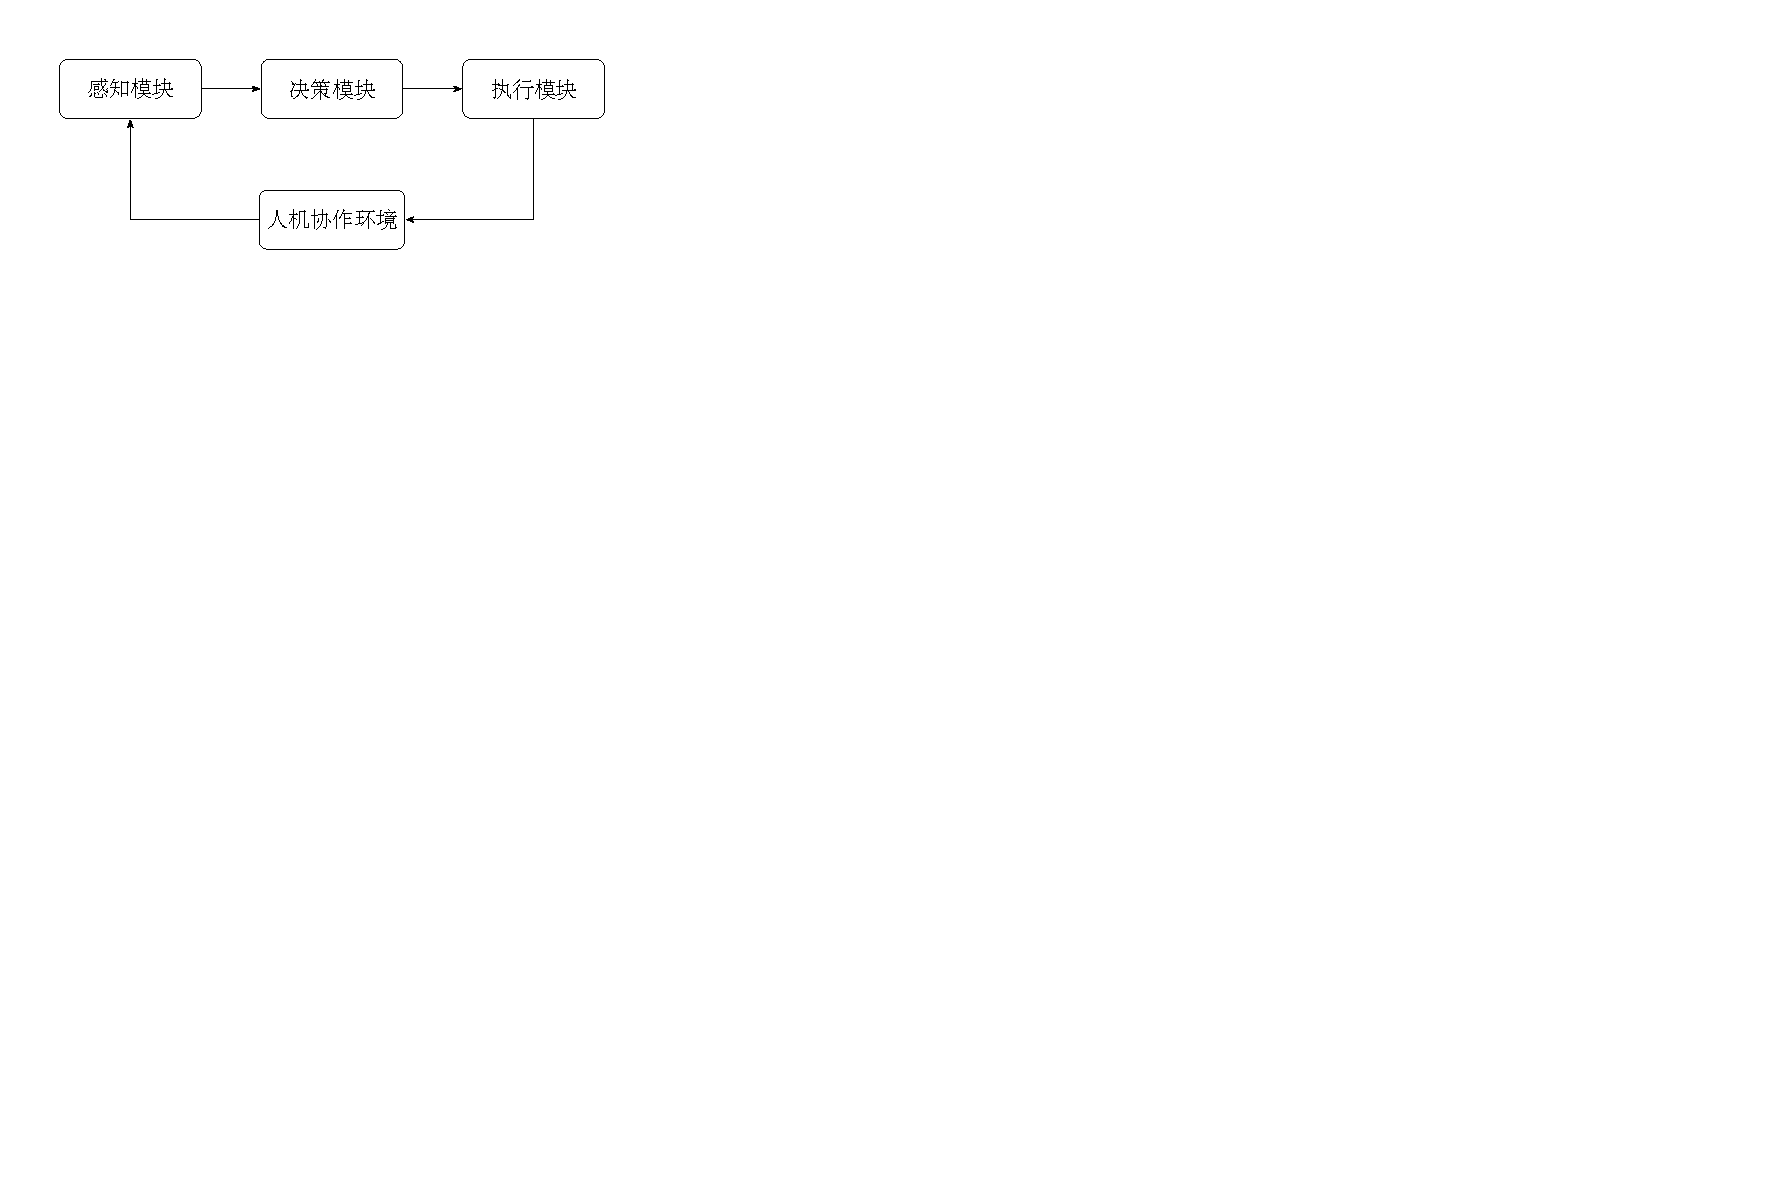
\includegraphics[width=0.7\textwidth]{figures/example-figure.pdf}
  \caption{示例插图——方法总体框架}
  \label{fig:framework}
\end{figure}

\subsection{微调衰减现象}
% TODO: E0–E2 衰减曲线族，双威胁模型下的现象观察（本章 motivation 图）。

\subsection{基于梯度投影的衰减机理}
% TODO: 梯度投影能量假设；正交补投影干预的因果验证。

\subsection{方法总体框架}
% TODO: 三重损失目标函数 L_total = L_forget + λ1·L_orth + λ2·L_drift；总体框架图。

\subsection{梯度正交约束设计}
% TODO: 代理微调梯度子空间估计；锚点一律取编辑后快照 θ_edit。

\subsection{编辑锚定方法谱系}
% TODO: 软锚定 / 硬锚定 / 预加固方法谱系；算法伪代码与复杂度分析。

\section{实验结果与分析}

\subsection{实验设置}
% TODO: 数据集（SafeEdit、OR-Bench/XSTest、Alpaca/GSM8K/CodeAlpaca、去拒答对抗数据）；
%       模型（Llama-2-7b-chat、Mistral-7B-Instruct）；基线与超参数设置。

\subsection{编辑保持率对比分析}
% TODO: E0–E2 基线衰减曲线 + E3–E5 定向锚定主结果 + E8 ILU 范式对比。

\subsection{消融实验}
% TODO: E6 软硬锚定谱系对比；E7 定向加权 vs 均匀正则消融。

\subsection{通用能力影响分析}
% TODO: 过度拒绝率、MMLU、新知识学习率——证明锚定不阻碍微调学习新知识。

\section{本章小结}
本节为示例占位内容。请替换为本章的小结。
